\section{Approach Overview} \label{sec:overview}

\begin{figure*}
\centering
  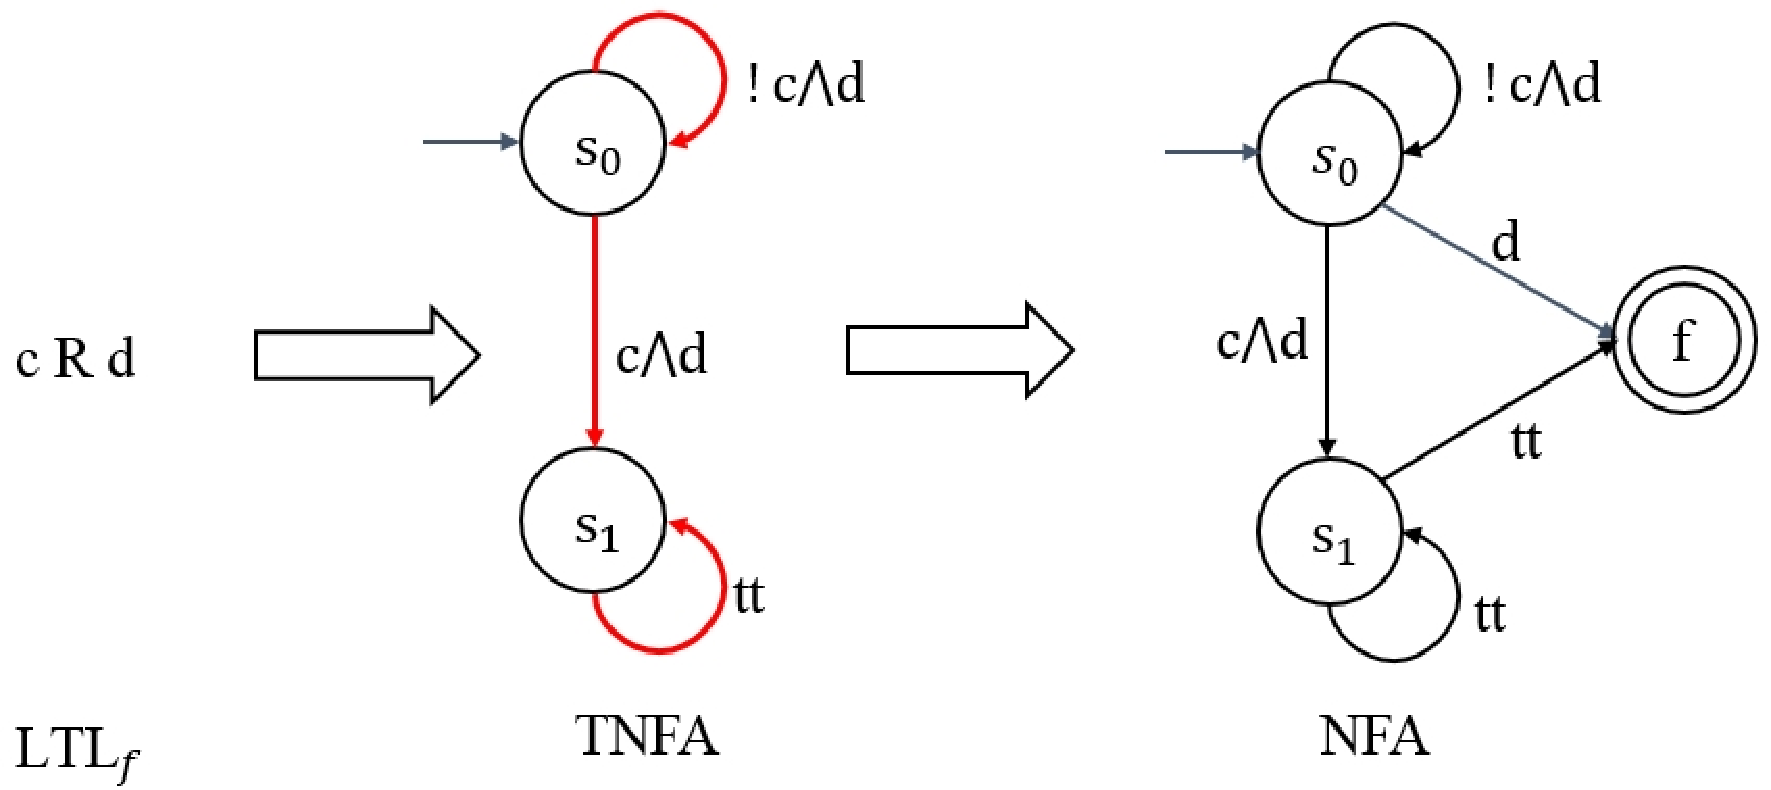
\includegraphics[scale=0.4]{overview.pdf}
  \caption{An example of our approach to construct the \NFA from an \ltlf formula. From left to right, the figure displays the input formula ($c\R d$), the equivalent transition-based \NFA (\TNFA) and the equivalent \NFA respectively. The red transitions in the \TNFA are accepting transitions.}
  \label{fig:overview}
\end{figure*}

Our approach first constructs the equivalent transition-based \NFA (\TNFA) for the input formula and then converts the \TNFA to its equivalent \NFA. A \TNFA is a special \NFA whose accepting conditions are defined over transitions instead of states. To convert a \TNFA to its equivalent \NFA, one can create a new state $f$ and add the transition $s\tran{\omega}f$ into the result \NFA for every accepting transition $s\tran{\omega}s'$ in the \TNFA. The new state $f$ is the only accepting state in the result \NFA. Figure \ref{fig:overview} illustrates an example of the whole translation process. 

Given an \ltlf formula $\phi$, the high-level descriptions on how to generate the equivalent \TNFA are as follows. We first convert $\phi$ to its neXt Normal Form (\XNF), which can be considered as a propositional formula over the alphabet composed of only Boolean atoms and neXt formulas. For example, the \XNF of the formula $\phi=a\R b$, which is denoted as $\xnf(\phi)$, is $b\wedge (a\vee \X(a\R b))$. Notably, the conversion cost from an \ltlf formula to its \XNF is linear to the size of the formula. Then we denote $\xnf(\phi)^p$ is the propositional formula over the alphabet set $\{a, b, \X(a\R b)\}$.

Taking $\xnf(\phi)^p$ as the input, an \SAT solver is able to compute a satisfying assignment $A$, e.g., $A=\{\neg a, b, \X(a\R b)\}$. The information inside $A$ indicates that there is a transition from $\phi$ to itself with the label $\neg a\wedge b$. Analogously, the assignment $A=\{a, b, \neg \X(a\R b)\}$ tells that there is a transition from $\phi$ to $\tt$ (because there is no $\X$ element in $A$) with the label $a\wedge b$. Now $\tt$ is a new state and we continue the above process to create new transitions until no new state is generated. Finally we identify the accepting transitions, the details of which are shown below. 

Constructing the equivalent \DFA from an \ltlf formula is similarly to that for \NFA. We can also utilize the \SAT techniques to obtain a transition-based \DFA (\TDFA) directly from the input formula. The idea to generate deterministic transitions are as follows. For the given state $q$, which essentially is a set of set of subformulas of the input formula and can be considered as a formula as well, we use the \SAT solver to get one of the satisfying assignment $A$ of $\xnf(q)^p$ at first. From $A$ we can fix the label, denoted as $L(A)$, on the transition and then enumerate all satisfying assignments of $q$ that includes $L(A)$. After that, we create a transition starting from $q$ with the label $L(A)$. Recursively applying the above procedure, all the states of the $\TDFA$ can be constructed. Finally, we present a methodology to identify the accepting transitions on the generated automaton, whose details are as below. 

From the \TDFA we can easily construct the equivalent \NFA, from which one can use the Subset Construction to create the corresponding \DFA.




